\documentclass[tikz,border=2pt]{standalone}
\usepackage[T1]{fontenc}
\usepackage{libertine}
\usepackage{xcolor}
\usetikzlibrary{arrows.meta}

\begin{document}
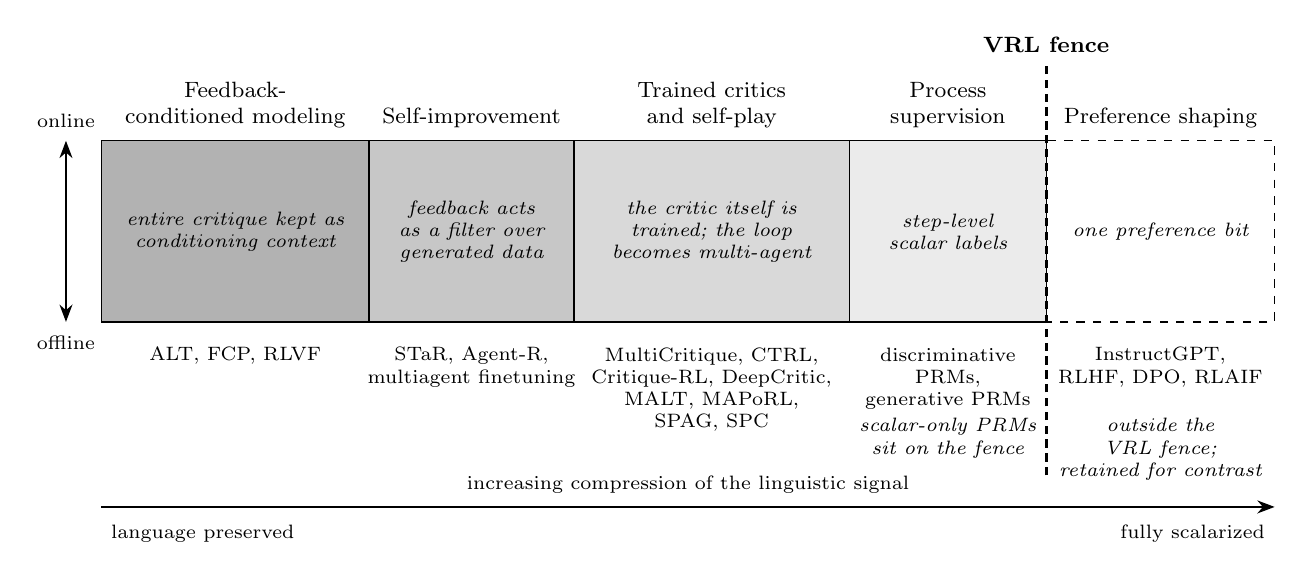
\begin{tikzpicture}[
    font=\footnotesize,
    fam/.style={anchor=south, align=center, font=\footnotesize, inner sep=1pt},
    sig/.style={align=center, font=\scriptsize\itshape, inner sep=1pt},
    meth/.style={anchor=north, align=center, font=\scriptsize, inner sep=2pt},
    >={Stealth[length=2.2mm]}
]
    \fill[black!30] (1.0,0)  rectangle (4.4,2.3);
    \fill[black!22] (4.4,0)  rectangle (7.0,2.3);
    \fill[black!15] (7.0,0)  rectangle (10.5,2.3);
    \fill[black!8]  (10.5,0) rectangle (13.0,2.3);
    \draw[black, line width=0.5pt] (1.0,0) rectangle (13.0,2.3);
    \draw[black, line width=0.5pt] (4.4,0) -- (4.4,2.3);
    \draw[black, line width=0.5pt] (7.0,0) -- (7.0,2.3);
    \draw[black, line width=0.5pt] (10.5,0) -- (10.5,2.3);
    \draw[black, line width=0.5pt, dashed] (13.0,0) rectangle (15.9,2.3);

    \node[fam, text width=3.15cm] at (2.70,2.42)  {Feedback-conditioned modeling};
    \node[fam, text width=2.35cm] at (5.70,2.42)  {Self-improvement};
    \node[fam, text width=3.25cm] at (8.75,2.42)  {Trained critics\\and self-play};
    \node[fam, text width=2.30cm] at (11.75,2.42) {Process\\supervision};
    \node[fam, text width=2.65cm] at (14.45,2.42) {Preference shaping};

    \node[sig, text width=3.10cm] at (2.70,1.15)  {entire critique kept as conditioning context};
    \node[sig, text width=2.35cm] at (5.70,1.15)  {feedback acts as a filter over generated data};
    \node[sig, text width=3.20cm] at (8.75,1.15)  {the critic itself is trained; the loop becomes multi-agent};
    \node[sig, text width=2.30cm] at (11.75,1.15) {step-level scalar labels};
    \node[sig, text width=2.65cm] at (14.45,1.15) {one preference bit};

    \node[meth, text width=3.20cm] at (2.70,-0.25)  {ALT, FCP, RLVF};
    \node[meth, text width=2.75cm] at (5.70,-0.25)  {STaR, Agent-R,\\multiagent finetuning};
    \node[meth, text width=3.30cm] at (8.75,-0.25)  {MultiCritique, CTRL,\\Critique-RL, DeepCritic,\\MALT, MAPoRL,\\SPAG, SPC};
    \node[meth, text width=2.30cm] at (11.75,-0.25) {discriminative PRMs,\\generative PRMs};
    \node[meth, text width=2.70cm] at (14.45,-0.25) {InstructGPT, RLHF, DPO, RLAIF};
    \node[meth, font=\scriptsize\itshape, text width=2.40cm] at (11.75,-1.15)
        {scalar-only PRMs\\sit on the fence};
    \node[meth, font=\scriptsize\itshape, text width=2.90cm] at (14.45,-1.15)
        {outside the VRL fence;\\retained for contrast};

    \draw[black, line width=0.9pt, dash pattern=on 3pt off 2pt] (13.0,-1.95) -- (13.0,3.25);
    \node[anchor=south, font=\footnotesize\bfseries] at (13.0,3.30) {VRL fence};
    \draw[<->, line width=0.6pt] (0.55,0) -- (0.55,2.3);
    \node[anchor=south, font=\scriptsize] at (0.55,2.35)  {online};
    \node[anchor=north, font=\scriptsize] at (0.55,-0.05) {offline};
    \draw[->, line width=0.7pt] (1.0,-2.35) -- (15.9,-2.35);
    \node[anchor=south, font=\scriptsize] at (8.45,-2.30)
        {increasing compression of the linguistic signal};
    \node[anchor=north west, font=\scriptsize] at (1.0,-2.45)  {language preserved};
    \node[anchor=north east, font=\scriptsize] at (15.9,-2.45) {fully scalarized};
\end{tikzpicture}
\end{document}
